\subsection{Image Segmentation}
Image segmentation is an effective means of isolating an object from its background and has been successfully used for different applications \cite{b4_1,b4_2,b4_3}. We perform segmentation with 2 segmentation masks -- one for lighter vegetables and one for darker vegetables. The values for the masks (see Table \ref{tab:mask_vals}) are selected experimentally based on their performances on the training images.

\bgroup
\def\arraystretch{1.5}
\begin{table}[htbp]
	\caption{Treshold Values for Segmentation Masks}
	\begin{center}
		\begin{tabular}{|c|c|c|c|c|}
			\hline
			& \multicolumn{4}{c|}{\textbf{Colour}}                                                         \\ \cline{2-5} 
			\multirow{-2}{*}{\textbf{Mask}} & \multicolumn{2}{c|}{\textbf{Lower Treshold}} & \multicolumn{2}{c|}{\textbf{Upper Treshold}}  \\ \hline
			Light Vegetable Mask            & RGB(0, 40, 40)   & \cellcolor[HTML]{002828}  & RGB(240, 240, 240) & \cellcolor[HTML]{F0F0F0} \\ \hline
			Dark Vegetable Mark             & RGB(0, 80, 80)   & \cellcolor[HTML]{005050}  & RGB(255, 255, 255) & \cellcolor[HTML]{FFFFFF} \\ \hline
		\end{tabular}
		\label{tab:mask_vals}
	\end{center}
\end{table}
\egroup

Once the two masks are applied to an image, they are downsampled with max-pooling to 25\% of the original size as illustrated in Fig. \ref{fig:mask}. We do this to reduce the computational complexity of learning and to make the model more tolerant to slight displacements. The resultant image is used as an input for the classifier discussed in section \ref{classifiers}.

\begin{figure}[tp]
	\centerline{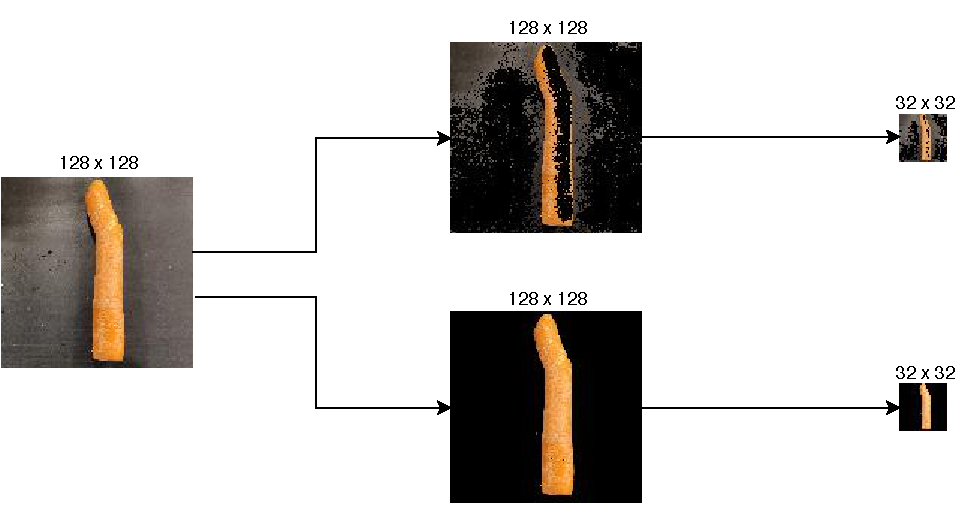
\includegraphics[scale=0.5]{./img/mask.pdf}}
	\caption{The steps to extract masked downsampled data.}
	\label{fig:mask}
\end{figure}

\subsection{Feature Extraction}
In addition to segmentation, additional attributes and characteristics of the vegetables are extracted with feature extraction methods \cite{b4_4}. We use LBP and HOG to get the textures and shapes of the vegetables respectively. As shown in Fig. \ref{fig:lbp_hog}, both feature extractions are applied to the 2 masked images before they are max-pooled. We do this to retain a high quality for feature extraction while focusing on only the object of interest without its background.

\begin{figure}[tp]
	\centerline{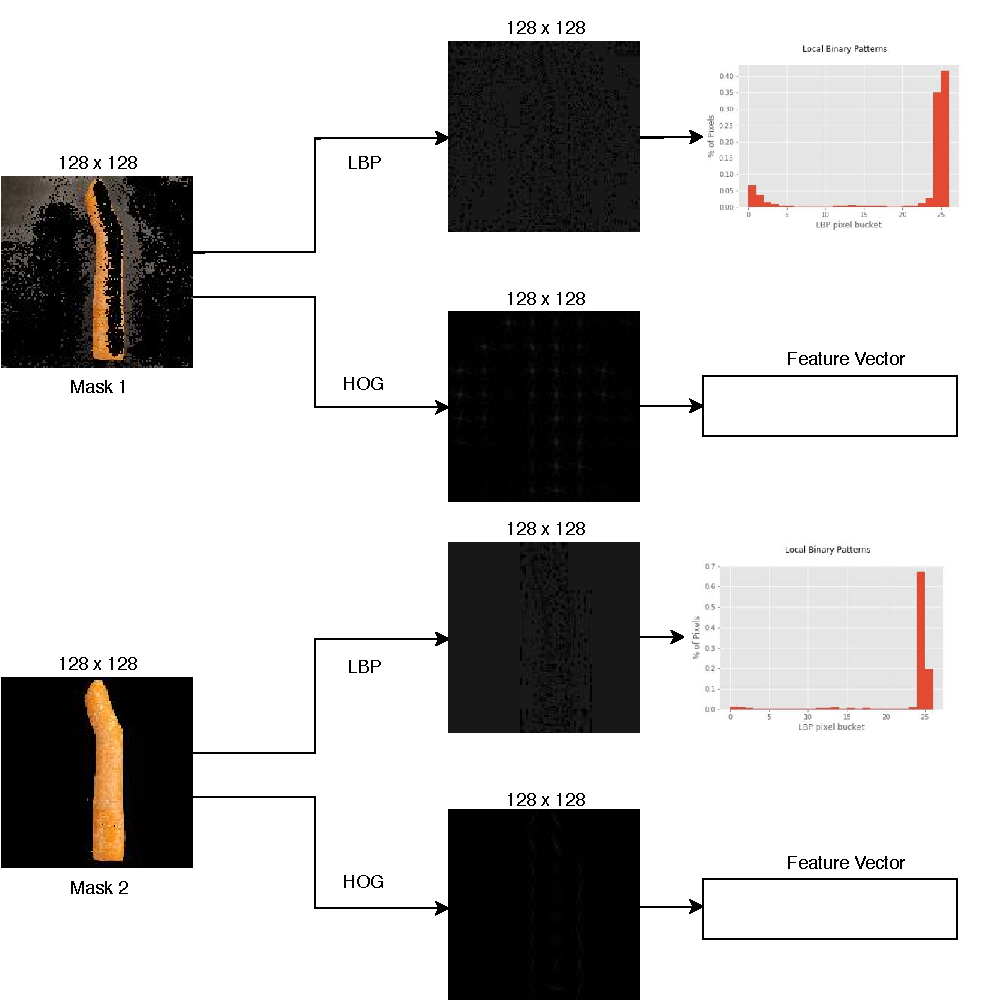
\includegraphics[scale=0.5]{./img/lbp_hog.pdf}}
	\caption{The steps to extract LBP and HOG feature vectors.}
	\label{fig:lbp_hog}
\end{figure}